\begin{frame}{Slave Motor (Right)}
	\framesubtitle{Setpoint Characteristic}
  \begin{itemize}
		\item Feeds the metal strip
		\item Lower Velocity
	\end{itemize}

		\centering
			\includegraphics[height=0.5\textheight]{RM_RPM_Current.png}
	\end{frame}

\begin{frame}{Slave Motor}
  \framesubtitle{Identification}


\begin{equation}
	RM(s) \simeq \frac{7.128}{6.0665s+1}
\end{equation}



			\centering
				\includegraphics[width=.9\textheight]{RM_systemID.png}


\end{frame}

\begin{frame}{Slave Motor}
  \framesubtitle{Controller Choice}
  \begin{block}{P Controller}
	\begin{itemize}
		\item Fast response, better tracking than PI
		\item Steady state error rejection not necessary due to cascade control
	\end{itemize}
  \end{block}
\end{frame}


	\begin{frame}{Slave Motor}
  \framesubtitle{Controller Tuning}

		\centering
			\includegraphics[height=.7\textheight]{RM_rlocus}



	\end{frame}


\begin{frame}{Slave Motor}
\framesubtitle{Simulation -- $K_P = 3$}
\centering
\includegraphics[width = \textwidth]{RM_K3_SIM.png}
\end{frame}



\begin{frame}{Slave Motor}
\framesubtitle{Verification -- $K_P = 2$ }
\centering
\includegraphics[width = \textwidth]{RM_K2.png}
\end{frame}


\begin{frame}{Slave Motor}
\framesubtitle{Verification -- $K_P = 3$}
\centering
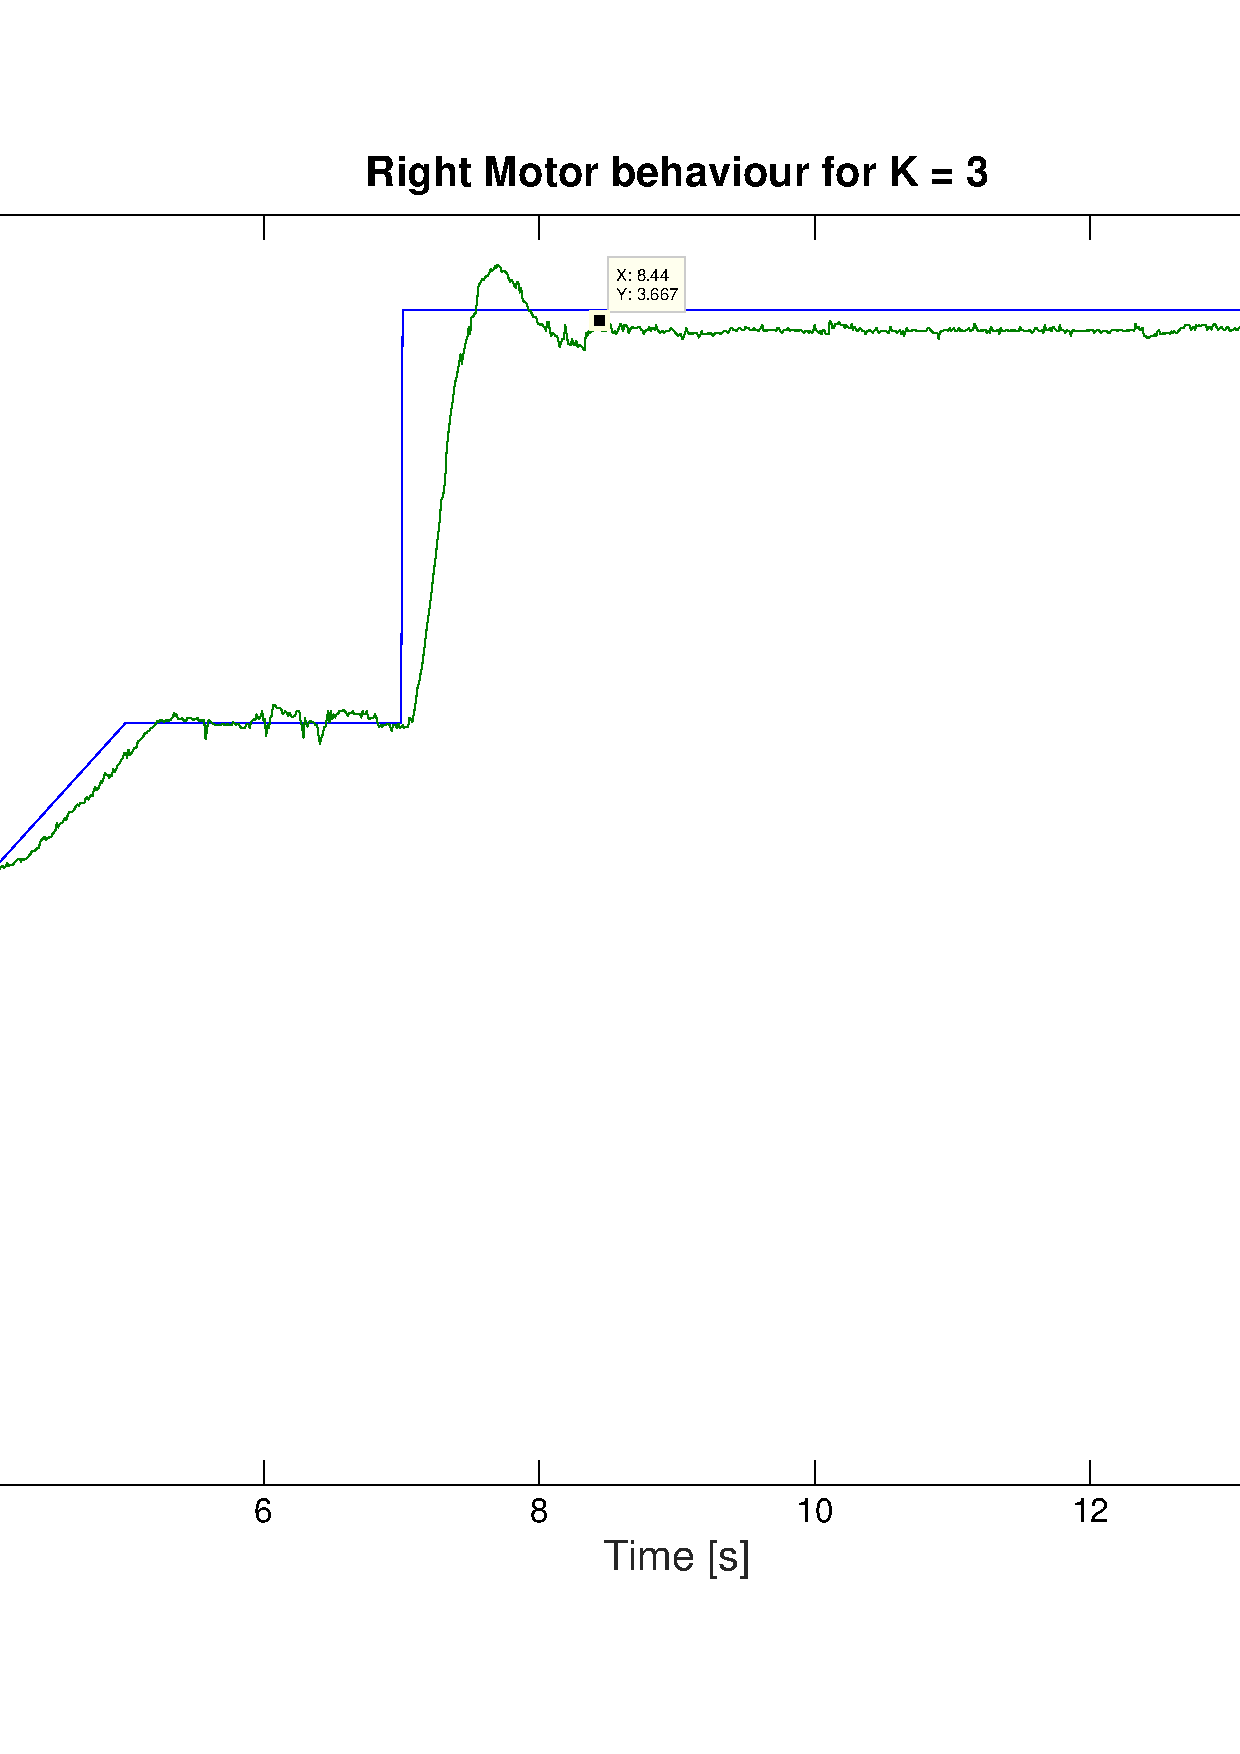
\includegraphics[width = \textwidth]{RM_K3.png}
\end{frame}


\begin{frame}{Slave Motor}
\framesubtitle{Verification -- $K_P = 4$}
\centering
\includegraphics[width = \textwidth]{RM_K4.png}
	\end{frame}

\begin{frame}{Slave Motor}
\framesubtitle{Conclusion}
\begin{block}{Final tuning}
\begin{itemize}
\item P Controller for fast tracking
\item Gain $K_P = 3$ to avoid actuator saturation
\item Overshoot is due to non linearities and higher order effects
\end{itemize}
\end{block}
\begin{block}{Closed loop experimental response}
\[Slave(s) \simeq \frac{0.9577}{0.2428s + 1}\]
\end{block}
\end{frame}
